\documentclass[handout]{beamer} % [handout] para imprimir eliminando transiciones

%\usefonttheme[onlymath]{serif}
%\usepackage{fontspec}
%\defaultfontfeatures{Mapping=tex-text}
%\setsansfont[Ligatures={Common}]{Futura}
%\setmonofont[Scale=0.8]{Monaco} 

\usepackage{beamerthemesplit}
\usepackage[utf8]{inputenc}
\usepackage[spanish]{babel}
\mode<presentation>
\usetheme{default}
\usecolortheme{dolphin}
\usepackage{alltt}                                    % \begin{alltt}
\usepackage{amssymb}                                  % mathematical symbols
\usepackage{comment}
\usepackage{tabto}                                    % \tabto
\usepackage{tikz}
\usetikzlibrary{automata}
\usetikzlibrary{positioning}
\usetikzlibrary{calc}

\usepackage{verbatim}                                 % comentarios

\title{Lenguajes de Programación}                     %[titulo corto]
\author{Fabián Riquelme Csori}                        %[nombre corto]
\date{2017}                                           %[fecha corta]
\institute{Universidad de Valparaíso}                 %[instituto corto]

\newcommand{\HRule}{\rule{\linewidth}{0.2mm}\\[1ex]}
\newcommand{\blue}[1]{\textcolor{blue}{#1}}
\newcommand{\red}[1]{\textcolor{red}{#1}}
\newcommand{\redb}[1]{{\color{red!70!black}{#1}}}
\newcommand{\green}[1]{{\color{green!70!black}{#1}}}
\newcommand{\gray}[1]{{\color{gray!50!white}{#1}}}
\newcommand{\lQ}{\mbox{``}}
\newcommand{\rQ}{\mbox{''}}
% \alert{texto destacado en rojo}
% \color{green} Color en verde
% \structure{texto en lila}


\begin{document}

%\begin{frame}%[plain]
%  \titlepage
%\end{frame}
%
% [opciones]:
% plain: oculta barra de navegacion, deja + espacio para contenido
% fragile: usar comandos como verbatim
% b,c,t: alineacion vertical
% label=nombre_etiqueta
% allowframebreaks: divide contenido en varios frames si es demasiado largo
% shrink: para escribir mucho texto en una transparencia, reduciendo tamano de fuente

%%%%%%%%%% PORTADA %%%%%%%%%%
\begin{frame}[plain]
  \begin{figure}[h]
    \begin{minipage}{0.3\textwidth}
    
\includegraphics[width=.9\textwidth]{./image/logo-UV.png}
    \end{minipage}
    \begin{minipage}{0.65\textwidth}
     $~$\\[3.6ex]
     \footnotesize{Escuela de Ingeniería Civil Informática}\\
     \footnotesize{Facultad de Ingeniería}
    \end{minipage}
  \end{figure}
  \begin{center}
    \vspace{1ex}
    \HRule
    \Large{Lenguajes de Programación}\\{\small Capítulo II: Análisis léxico y sintáctico}\\[-1ex]
    \HRule\vspace{1ex}
    \large{Fabián Riquelme Csori}\\[.5ex]\footnotesize{fabian.riquelme@uv.cl}\\[6ex] {\tiny 2017-II}\\[6ex]
  \end{center}
\end{frame}

%%%%%%%%%% INDEX %%%%%%%%%%
\begin{frame}
 \frametitle{Index}
 \scriptsize 			% reducir tamano de letra
 \tableofcontents		%[pausesections]
\end{frame}

%%%%%%%%%%% ACTUAL INDEX %%%%%%%%%%
%\AtBeginSection[] %generar indice automaticamente
%{
%\begin{frame}<beamer>%[plain]
% \frametitle{Index}
% \framesubtitle{subtitulo}
% \scriptsize
% \tableofcontents[currentsection, currentsubsection]
%\end{frame}
%}

%==============================
\section{Análisis léxico}

\begin{frame}{Primera fase de compilación}
    \begin{center}
    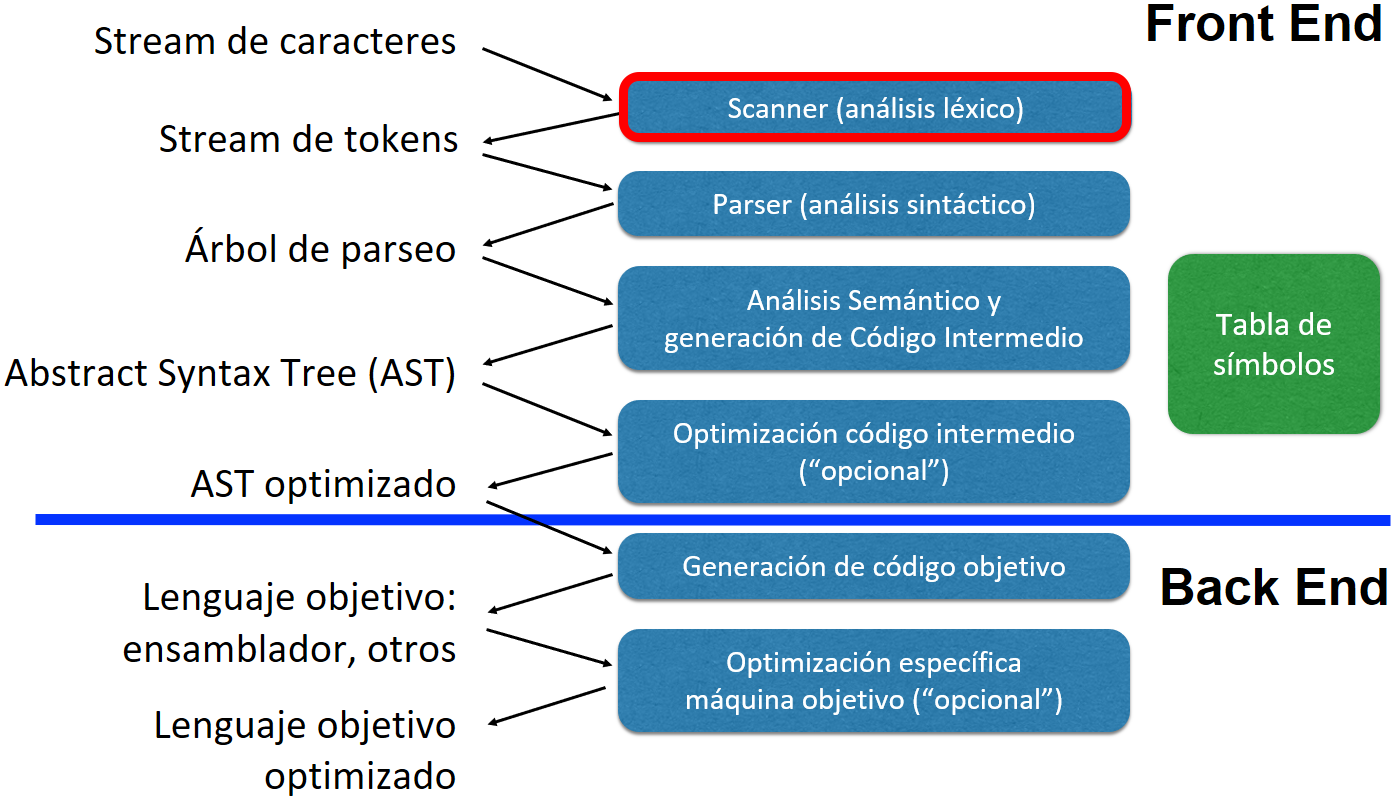
\includegraphics[width=\textwidth]{./image/cap2/compilador-fase1}
    \end{center}
\end{frame}

\begin{frame}{Léxico vs. sintaxis}
    Dado un lenguaje (de programación):
    \begin{itemize}
        \item<1-> Su \blue{léxico} es el conjunto de palabras que lo conforman\\
        (su diccionario).
        \begin{itemize}
            \item<2-> El \blue{analizador léxico} o \blue{scanner} de un compilador verifica que los strings del código fuente sean válidos.
        \end{itemize}
        \item<3-> Su \blue{sintaxis} es el conjunto de reglas que definen sus secuencias de strings válidas.
        \begin{itemize}
            \item<4-> El \blue{analizador sintáctico} o \blue{parser} de un compilador verifica que los strings (válidos) del código fuente estén escritos en el orden correcto.
        \end{itemize}
        \item<5-> Tanto el léxico como las reglas sintácticas deben ser precisas y no ambiguas, por lo que se requiere de un método formal de notación.
    \end{itemize}
\end{frame}

%------------------------------
\subsection{Expresiones regulares}

\begin{frame}{Ejemplo: números naturales}
    Un \blue{número} es una concatenación de \blue{dígitos}, donde el primer dígito es distinto de \blue{cero}.
    \begin{itemize}
        \item<2-> Ej: ``7645'' = ``7'' + ``6'' + ``4'' + ``5''
        \item<3-> Pero también hay números que tienen ceros:\\
        Ej: ``76405'' = ``7'' + ``6'' + ``4'' + ``0'' + ``5''
    \end{itemize}
    \uncover<4->{¿Cómo definir un patrón general para diferenciar números de strings arbitrarios?}
\end{frame}

\begin{frame}{Refresquemos la memoria...}
    \begin{itemize}
        \item<1-> Un \blue{alfabeto} $\Sigma$ es un conjunto finito y no vacío de símbolos o caracteres.
        \item<2-> Un \blue{string} o \blue{cadena de caracteres} es una secuencia finita de símbolos de un alfabeto, $x\in\Sigma^*$.
        \begin{itemize}
            \item<3-> $\varepsilon\in\Sigma^*$ es el \blue{string vacío} ($\varepsilon\notin\Sigma$).
        \end{itemize}
        \item<4-> Un \blue{lenguaje} es un conjunto (posiblemente infinito) de strings, $L\subseteq\Sigma^*$.
        \item<5-> Una \blue{expresión regular} es una notación formal para denotar un lenguaje.
    \end{itemize}
\end{frame}

\begin{frame}{Expresiones regulares}
    Sean $E$, $E_1$ y $E_2$ expresiones regulares sobre un alfabeto $\Sigma$.\\
    Una \blue{expresión regular} (RE) se puede definir recursivamente:
    \begin{itemize}
        \item<2-> $\forall x\in\Sigma$, $x$ es una RE.
        \item<3-> $\varepsilon$ es una RE.
        \item<4-> $E_1\mid E_2=\{x\mid x\in E_1\vee x\in E_2\}$ es una RE (Disyunción)
        \item<5-> $E_1\cdot E_2=\{xy\mid x\in E_1\wedge y\in E_2\}$ es una RE (Concatenación)\\
        \uncover<6->{(la concatenación de $k$ veces $E$ consigo misma se denota $E^k$).\\}
        \uncover<7->{(note que $E^0=\{\varepsilon\}$)}
        \item<8-> $E^*=\bigcup_{k\geq 0}E^k$ es una RE (Clausura de Kleene)
    \end{itemize}
    \uncover<9->{Para establecer órdenes de precedencia y evitar ambigüedades, podemos utilizar paréntesis.}
\end{frame}

\begin{frame}{Expresiones regulares}
    \begin{block}{Ejemplos}
      \begin{itemize}
          \item<1-> $a\mid b=$\uncover<2->{$\{\lQ a\rQ,\lQ b\rQ\}$}
          \item<3-> $(a\mid b)\cdot a=$\uncover<4->{$\{\lQ aa\rQ,\lQ ba\rQ\}$}
          \item<5-> $(a\cdot b)\mid\varepsilon=$\uncover<6->{$\{\lQ ab\rQ,\lQ~\rQ\}$}
          \item<7-> $((a\mid b)\cdot a)^*=$\uncover<8->{$\{\lQ~\rQ, \lQ aa\rQ,\lQ aaaa\rQ,\lQ ba\rQ,\lQ baba\rQ,\ldots\}$}
      \end{itemize}
    \end{block}
\end{frame}

\begin{frame}{Notación adicional}
    \begin{itemize}
        \item<1-> Podemos omitir el operador de concatenación y epsilon
        \item<2-> El operador $^*$ tiene más precedencia que operador $\cdot$
        \item<2-> El operador $\cdot$ tiene más precedencia que operador $\mid$
        \item<3-> Los corchetes cuadrados [ ] permiten abreviar la disyunción.\\
        Ej: [$abcd$] = $a\mid b\mid c\mid d$
        \item<4-> $E^+=(E\cdot E^*)$
        \item<4-> $E?=(E\mid\varepsilon)$
        \item<5-> Podemos usar rangos de caracteres, cuando el contexto lo permite.
        Ej: [$b$-$g$] = [$bcdefg$]
    \end{itemize}
\end{frame}


%------------------------------
\subsection{Tokens y autómatas finitos}

\begin{frame}{Tokens y RE}
    Un \blue{token} es una secuencia de caracteres que puede ser tratada como una unidad en la gramática de un lenguaje de programación.\\
    \pause
    \begin{block}{Ejemplos}
    \begin{itemize}
        \item<2-> DIGITO := [0-9]
        \item<3-> DIGITO\_NO\_CERO := [1-9]
        \item<4-> NATURAL := DIGITO\_NO\_CERO DIGITO$^*$
        \item<5-> BIN\_OP := $+\mid -$
    \end{itemize}
    \end{block}
    \uncover<6->{Los dígitos reconocidos no tienen significado, \blue{sólo son símbolos}.}\\
    \uncover<7->{El análisis léxico de un programa consiste en construir un \blue{flujo de tokens} que será consumido por el analizador sintáctico.}
\end{frame}

\begin{frame}{Tokens y RE}
    Un lenguaje clasifica los tokens léxicos en un conjunto finito de \blue{tipos de token}.
    \pause
    \begin{center}
      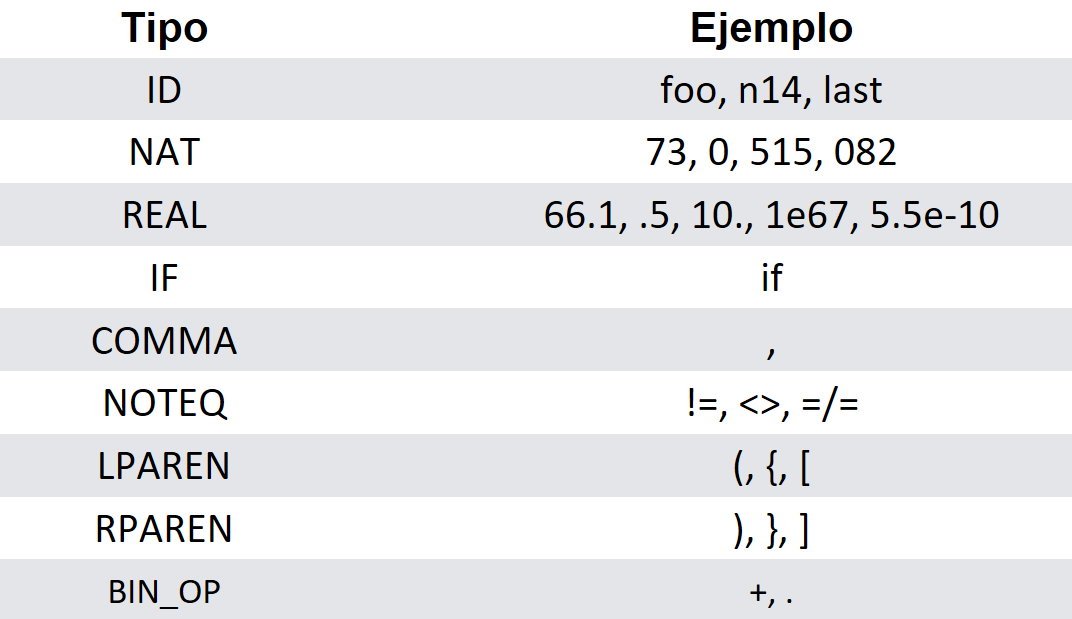
\includegraphics[width=.8\textwidth]{./image/cap2/tipos-token}
    \end{center}
\end{frame}

\begin{frame}{Autómatas finitos (FA)}
  $(a\mid ba\mid bba)^*(\varepsilon\mid b\mid bb)$
  \begin{center}
    \begin{tikzpicture}  
      \node[state,initial,accepting,initial text = Inicio] (q_0)                {$q_0$};
      \node[state,accepting]                               (q_1) [right=of q_0] {$q_1$};
      \node[state,accepting]                               (q_2) [right=of q_1] {$q_2$};
      \node[state]                                         (q_3) [below=of q_2] {$q_3$};
  
      \path[->,thick] (q_0) edge node[above] {$b$} (q_1)
			                edge [loop above] node {$a$} ()
		              (q_1) edge [bend left] node[above] {$a$} (q_0)                         
			                edge node[above] {$b$} (q_2)
		              (q_2) edge [bend left] node[below] {$a$} (q_0)
		                    edge node[right] {$b$} (q_3)
                      (q_3) edge [loop left] node[above = 3pt] {$a,b$} (); 
    \end{tikzpicture} 
  \end{center}
\end{frame}

\begin{frame}{Autómatas finitos deterministas (DFA)}
  Un \blue{autómata finito determinista} (\blue{DFA}) es una tupla $A=(Q,\Sigma,\delta,s,F)$ tal que:
 \begin{itemize}
  \item $Q$ es un conjunto finito de estados.
  \item $\Sigma$ es un alfabeto finito.
  \item $s\in Q$ es el estado inicial.
  \item $F\subseteq Q$ es el conjunto de estados finales.
  \item $\delta:Q\times\Sigma \to Q$ es la función de transición.
 \end{itemize}
\end{frame}

\begin{frame}{Autómatas finitos deterministas (DFA)}
  \begin{center}
    \begin{tikzpicture}
      \node[state,initial,initial text = Inicio]   (q_0)                {$q_0$};
      \node[state,accepting]                       (q_1) [right=of q_0] {$q_1$};
  
      \path[->,thick] (q_0) edge [bend left] node[above] {$b$} (q_1)
	                        edge [loop above] node {$a$} ()
		              (q_1) edge [loop above] node {$a$} ()
			                edge [bend left] node[above] {$b$} (q_0);
    \end{tikzpicture} 
  \end{center}

  $Q = \{q_0,q_1\}, \Sigma = \{a,b\}, s = q_0, F = \{q_1\}$ y la función $\delta$:
  \begin{equation*}
    \begin{array}{c|cc}
      \delta & q_0 & q_1 \\ \hline
           a & q_0 & q_1 \\
           b & q_1 & q_0
    \end{array}
  \end{equation*}
\end{frame}

\begin{frame}{Autómatas finitos no-deterministas (NFA)}
  Un \blue{autómata finito no-determinista} (\blue{NFA}) es una tupla $A=(Q,\Sigma,\Delta,s,F)$ tal que:
  \begin{itemize}
      \item $\Delta\subset(Q\times\Sigma)\times Q$ es la \textit{relación} de transición, finita.
  \end{itemize}
  \pause
  
  Solo cambia $\delta$ por $\Delta$, que permite transiciones con $\varepsilon$.
  \pause
  \begin{block}{Ejemplo}
    $(ab\mid aba)^*$
    \begin{center}
      \begin{tikzpicture}
       \node[state,initial,accepting,initial text = Inicio] (q_0) {$q_0$};
       \node[state]                                         (q_1) [right=of q_0] {$q_1$};
       \node[state]                                         (q_2) [right=of q_1] {$q_2$};
       \path[->,thick] (q_0) edge node[above] {$a$} (q_1)                         
                       (q_1) edge node[above] {$b$} (q_2)
                       (q_2) edge [bend right] node[above] {$a$} (q_0)
                             edge [bend left] node[below] {$\varepsilon$} (q_0);
      \end{tikzpicture}   
   \end{center}
  \end{block}
  \pause
  ¡Recordar: Todo NFA puede transformarse a un DFA!
\end{frame}

%------------------------------
\subsection{Analizadores léxicos (Scanners)}

\begin{frame}{DFAs como analizadores léxicos}
    \begin{center}
      \begin{tikzpicture}
       \node[state,initial,initial text = Inicio] (q_0) {};
       \node[state,accepting]                     (q_1) [right=of q_0] {\tiny{NATURAL}};
       \node[state]                               (q_2) [right=of q_1] {};
       \path[->,thick] (q_0) edge node[above] {[0-9]} (q_1)
                       (q_1) edge node[above] {$+\mid -$} (q_2)
                       (q_1) edge [loop above] node {[0-9]} (q_1)
                       (q_2) edge [bend left] node[below] {[0-9]} (q_1);
      \end{tikzpicture}   
   \end{center}
   ``NATURAL'' es un token y un estado final.
   \medskip\pause
   
   \alert{Ejercicio}\\
   Modificar el DFA para que los naturales solo comiencen con 0.
\end{frame}

\begin{frame}{Analizadores léxicos en Racket}
    \begin{center}
      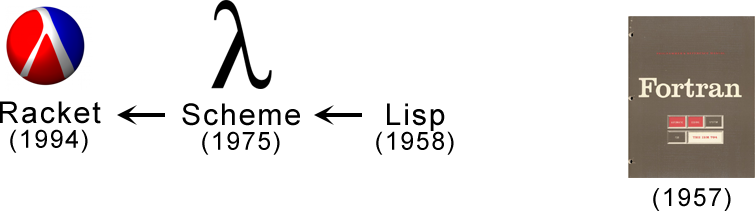
\includegraphics[width=.8\textwidth]{./image/cap2/racket-history}
      
      \url{https://docs.racket-lang.org/parser-tools/Lexers.html}
      \medskip
      
      \url{http://beautifulracket.com/}
    \end{center}
\end{frame}

%==============================
\section{Análisis sintáctico}

\begin{frame}{Segunda fase de compilación}
    \begin{center}
    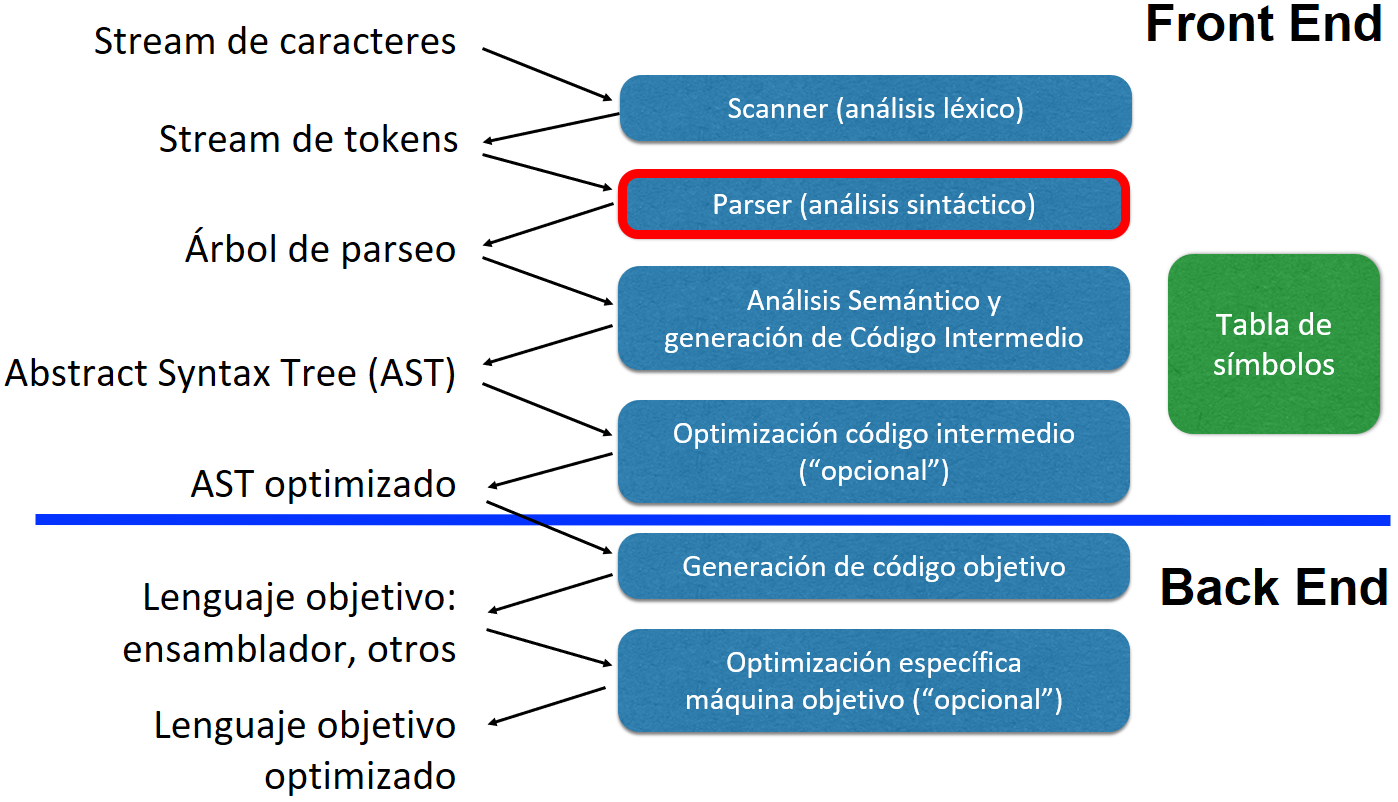
\includegraphics[width=\textwidth]{./image/cap2/compilador-fase2}
    \end{center}
\end{frame}

%------------------------------
\subsection{Gramáticas libres de contexto}

\begin{frame}{Ejemplo: Calculadora}
    ¿Cómo identificar y distinguir entre suma y resta?
    \begin{itemize}
        \item Ej: ``$7545 + 42$'' vs ``$7545 - 42$''
    \end{itemize}
    \pause
    
    La tokenización de ambos programas es:
    \begin{itemize}
        \item NATURAL(7545) BIN\_OP(+) NATURAL(42)
        \item NATURAL(7545) BIN\_OP(-) NATURAL(42)
    \end{itemize}
    \pause

    ¿Cómo definir un patrón general para los tipos de sintáxis que vemos en los lenguajes de programación?
\end{frame}

\begin{frame}{Ejemplo: Calculadora}
    Intentemos utilizar expresiones regulares:
    \begin{itemize}
        \item SUMA = (NATURAL ``+'')* NATURAL
    \end{itemize}
    \pause 
    
    Podemos enriquecer nuestro lenguaje con expresiones:
    \begin{itemize}
        \item SUMA = EXPR ``+'' EXPR
        \item EXPR = ``('' SUMA ``)'' $\mid$ NATURAL
    \end{itemize}
    \pause 
    
    Pero luego querremos escribir programas como:
    \begin{itemize}
        \item (109+23), 61, (1+(250+3)), etc...
    \end{itemize}
    \pause
    
    \textbf{Una expresión regular NO puede describir un lenguaje con una cantidad arbitraria de paréntesis balanceados.}
\end{frame}

\begin{frame}{Gramáticas Libres de Contexto (CFG)}
    Para la etapa de \blue{parsing}, los strings de un lenguaje están compuestos por símbolos de un \blue{alfabeto de tokens} (i.e., el conjunto de tokens retornado por el analizador léxico).
    \begin{itemize}
        \item<2-> Para el análisis léxico nos bastaba con un \blue{lenguaje regular}.
        \item<2-> Para el análisis sintáctico o parsing necesitamos un \blue{lenguaje libre de contexto}.
    \end{itemize}
    \uncover<3->{
    \begin{block}{Jerarquía de Chomsky}
    \smallskip
    
    {\small
      \begin{tabular}{c|l|l|l}\hline
        Tipo & Lenguaje & Autómata & Reglas prod. gramatical \\\hline
        0    & LRE      & Máquina de Turing
                        & $\alpha\to\beta$ (sin restricciones)\\
        1    & LSC      & A. linealmente acotado 
                        & $\alpha A\beta\to\alpha\gamma\beta$\\
        2    & LLC      & A. con pila
                        & $A\to\gamma$\\
        3    & LR       & A. finito
                        & $A\to aB$ o $A\to a$\\\hline
  \end{tabular}}
    \end{block}}
\end{frame}

\begin{frame}{Gramáticas Libres de Contexto (CFG)}
    \begin{block}{Ejemplo}
        $<$expr$>$ := NATURAL $\mid$ ``-'' $<$expr$>$\\
        $~~~~~~~~~~~~~$ $\mid$ ``('' $<$expr$>$ ``)'' $\mid$ $<$expr$>$ $<$op$>$ $<$expr$>$\\
        $<$op$>$ $~$ := BIN\_OP
    \end{block}
    \pause
    \begin{block}{Flujo de tokens}
        \begin{itemize}
            \item ``7545 + 42'' corresponde a:\\
                  NATURAL(7545) BIN\_OP(+) NATURAL(42)
            \item El token almacena el texto y otra información necesaria. Es decir, sabemos que $<$op$>$ = ``+''
            \item La pregunta es si esta sequencia de tokens corresponde a alguna derivación de $<$expr$>$
        \end{itemize}
    \end{block}
\end{frame}

\begin{frame}{Derivaciones gramaticales}
    \begin{itemize}
        \item<1-> Una secuencia de tokens pertenece a una gramática si es el producto de una serie de \blue{derivaciones} de la gramática.
        \item<2-> Partimos de la derivación inicial, buscando un posible calce. La única opción plausible es:
        \medskip
        
        $<$expr$>$ =$>$ $<$expr$>$ $<$op$>$ $<$\redb{expr}$>$\\
        $~~~~~~~~~~$ =$>$ $<$expr$>$ $<$\redb{op}$>$ NATURAL(42)\\
        $~~~~~~~~~~$ =$>$ $<$\redb{expr}$>$ BIN\_OP(+) NATURAL(42)\\
        $~~~~~~~~~~$ =$>$ NATURAL(7545) BIN\_OP(+) NATURAL(42)
    \end{itemize}
\end{frame}

\begin{frame}{Árbol de derivación}
    \begin{center}
    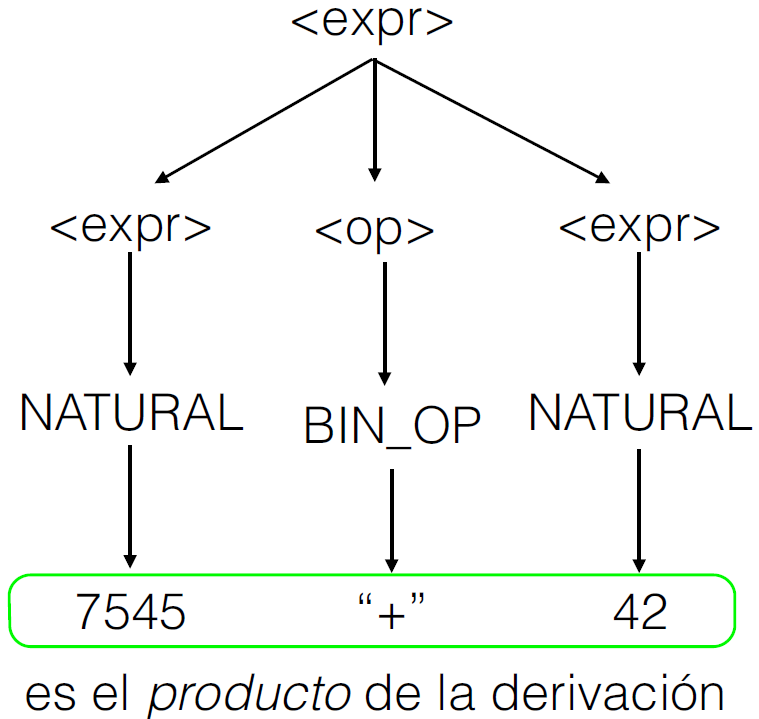
\includegraphics[width=.6\textwidth]{./image/cap2/arbol-derivacion}
    \end{center}
\end{frame}

\begin{frame}{Gramáticas ambiguas}
    \begin{itemize}
        \item<1-> Una gramática es \blue{ambigua} cuando un string posee más de un árbol de derivación posible.
        \item<2-> Por ejemplo, si $\varepsilon$ es el string vacío:
        \begin{center}$<$A$>$ := $<$A$>$ $\mid$ $\varepsilon$\end{center}
        es una gramática ambigua:
        \begin{itemize}
            \item A =$>$ $\varepsilon$
            \item A =$>$ A =$>$ A =$>$ $\ldots$ =$>$ A =$>$ $\varepsilon$
        \end{itemize}
        \item<3-> Muchos generadores de parsers aceptan gramáticas ambiguas y no ambiguas. En caso de ambigüedad, se utilizan ciertas heurísticas para decidir entre opciones igualmente aceptables.
    \end{itemize}
\end{frame}


%------------------------------
\subsection{Autómatas de pila}

\begin{frame}{Recordemos...}
    \begin{itemize}
        \item<1-> Los \blue{autómatas finitos deterministas} permiten analizar el \blue{léxico} de un lenguaje (\blue{scanner}) guiados por \blue{expresiones regulares}.
        \item<2-> Los \blue{autómatas de pila (deterministas)} permiten analizar la \blue{sintaxis} de un lenguaje (\blue{parser}) guiados por una \blue{gramática libre de contexto}.
    \end{itemize}
\end{frame}

\begin{frame}{Autómatas de pila deterministas (PDA)}
    $\{wcw^R\mid w\in \{a,b\}^*\}$
    \begin{center}
    \begin{tikzpicture}
        \node[state,initial,initial text = Inicio]   (q_0)                {$q_0$};
        \node[state,accepting]                       (q_1) [right=of q_0] {$q_1$};
  
        \path[->,thick] (q_0) edge node[above,text width=5ex] 
                                   {$c,a / $\\[-1ex]$c,b / $} (q_1)
		                	  edge [loop above] node[text width=6ex] 
		                	       {$a,a / a$\\$a,b / a$\\$a,~ / a$} ()
			                  edge [loop below] node[text width=6ex]
			                       {$b,a / b$\\$b,b / b$\\$b,~ / b$} ()
		                (q_1) edge [loop above] node {$a,a / $} ()
			                  edge [loop below] node {$b,b / $} ();
    \end{tikzpicture}
    \end{center}
\end{frame}

\begin{frame}{Autómatas de pila deterministas (PDA)}
  Un \blue{autómata de pila determinista} (\blue{PDA}) es una tupla $A=(Q,\Sigma,\Gamma,\delta,s,F)$ tal que:
 \begin{itemize}
  \item $Q$ es un conjunto finito de estados.
  \item $\Sigma$ es un alfabeto finito.
  \item $\Gamma$ es el alfabeto finito de la cinta.
  \item $s\in Q$ es el estado inicial.
  \item $F\subseteq Q$ es el conjunto de estados finales.
  \item $\delta: Q\times\Sigma^*\times\Gamma^* \to Q\times\Gamma^*$ es un conjunto finito de transiciones.
 \end{itemize}
\end{frame}

%------------------------------
\subsection{Analizadores sintácticos (Parsers)}

\begin{frame}{Lenguaje de programación Racket}
    \begin{itemize}
        \item<1-> Dada la especificación léxica y sintáctica de un lenguaje, usando expresiones regulares y CFG, respectivamente, es posible \blue{generar de manera automática} el scanner y parser correspondientes.
        \item<2-> Para ello se utilizan programas como \blue{flex} y \blue{bison} (en C), \blue{ANTLR} (en Java), o \blue{ml-lex} y \blue{ml-yacc} (en SML).
        \item<3-> También es posible definir scanners y parsers de manera manual. Esto puede ser por razones de eficiencia, o de legibilidad y comprensión del programa.
        \item<4-> Si la sintáxis es tan compleja que no puede expresarse como una CFG, se debe buscar otra alternativa de implementación.
    \end{itemize}
\end{frame}

\begin{frame}{Lenguaje de programación Racket}
    \begin{itemize}
        \item Lenguaje funcional (ya hablaremos de esto después)
        \item Notación prefija
        \begin{itemize}
            \item \begin{alltt}(function\_name par1 par2 ...)\end{alltt}
        \end{itemize}
        \item<2-> Lenguaje creado para construir lenguajes de programación:
        \begin{enumerate}
            \item Diseñar el \blue{reader}, que convierte un código fuente en \textit{S-expressions} de Racket (``analizador sintáctico'').
            \item Diseñar el \blue{expander}, que evalúa la sintaxis generada por el reader y le da sentido dentro del lenguaje de Racket (``analizador semántico'').
        \end{enumerate}
        \item<3-> Enlaces de ayuda
        \begin{itemize}
            \item \scriptsize{\url{https://docs.racket-lang.org/parser-tools/Lexers.html}}
            \item \scriptsize{\url{http://beautifulracket.com/}}
        \end{itemize}
    \end{itemize}
\end{frame}


%------------------------------

\begin{frame}
 \begin{block}{Bibliografía}
  \begin{itemize}
    \item Pratt, Terrence W. (1998). \textit{Lenguajes de programación: diseño e implementación}, Pearson Education.
    \item Sethi, Ravi (1992). \textit{Lenguajes de programación: conceptos y constructores}, Addison-Wesley Iberoamericana.
    \item Scott, Michael (2009). \textit{Programming Language Pragmatics}, Morgan Kaufman, 3ra ed.
  \end{itemize}
 \end{block}
 \begin{block}{Recursos}
  \begin{itemize}
    \item Apuntes de cursos anteriores (Ismael Figueroa).
    \item Wikipedia y Wikimedia Commons.
    \item Imágenes con licencia libre.
  \end{itemize}
 \end{block}
\end{frame}

\end{document}
